\documentclass[
	a4paper,
	oneside,
	BCOR = 10mm,
	DIV = 12,
	12pt,
	headings = normal,
]{scrartcl}

%%% Length calculations
\usepackage{calc}
%%%

%%% Support for color
\usepackage{xcolor}
\definecolor{lightblue}{HTML}{03A9F4}
\definecolor{red}{HTML}{F44336}
%%%

%%% Including graphics
\usepackage{graphicx}
%%%

%%% Font selection
\usepackage{fontspec}

\setromanfont{STIX Two Text}[
	SmallCapsFeatures = {LetterSpace = 8},
]

\setsansfont{IBM Plex Sans}[
	Scale = MatchUppercase,
]

\setmonofont{IBM Plex Mono}[
	Scale = MatchUppercase,
]
%%%

%%% Math typesetting
\usepackage{amsmath}

\usepackage{unicode-math}
\setmathfont{STIX Two Math}

\usepackage{IEEEtrantools}
%%%

%%% List settings
\usepackage{enumitem}
\setlist[enumerate]{
	label*      = {\arabic*.},
	leftmargin  = *,
	labelindent = \parindent,
	topsep      = 1\baselineskip,
	parsep      = 0\baselineskip,
	itemsep     = 1\baselineskip,
	noitemsep, % override itemsep
}

\setlist[itemize]{
	label*      = {—},
	leftmargin  = *,
	labelindent = \parindent,
	topsep      = 1\baselineskip,
	parsep      = 0\baselineskip,
	itemsep     = 1\baselineskip,
	noitemsep, % override itemsep
}

\setlist[description]{
	font        = {\rmfamily\upshape\bfseries},
	topsep      = 1\baselineskip,
	parsep      = 0\baselineskip,
	itemsep     = 0\baselineskip,
}

%%%

%%% Structural elements typesetting
\setkomafont{pagenumber}{\rmfamily\upshape}
\setkomafont{disposition}{\rmfamily\bfseries}

% Sectioning
\RedeclareSectionCommand[
	beforeskip = -1\baselineskip,
	afterskip  = 1\baselineskip,
	font       = {\normalsize\bfseries\scshape},
]{section}

\RedeclareSectionCommand[
	beforeskip = -1\baselineskip,
	afterskip  = 1\baselineskip,
	font       = {\normalsize\bfseries\itshape},
]{subsection}

\RedeclareSectionCommand[
	beforeskip = -1\baselineskip,
	afterskip  = 1\baselineskip,
	font       = {\normalsize\bfseries},
]{subsubsection}

\RedeclareSectionCommand[
	beforeskip = -1\baselineskip,
	afterskip  = -0.5em,
	font       = {\normalsize\mdseries\scshape\addfontfeatures{Letters = {UppercaseSmallCaps}}},
]{paragraph}
%%%

%%% Typographic enhancements
\usepackage{microtype}
%%%

%%% Language-specific settings
\usepackage{polyglossia}
\setmainlanguage{ukrainian}
\setotherlanguages{english}
%%%

%%% Captions
\usepackage{caption}
\usepackage{subcaption}

%\DeclareCaptionLabelFormat{closing}{#2)}
%\captionsetup[subtable]{labelformat = closing}

%\captionsetup[subfigure]{labelformat = closing}

\captionsetup[table]{
	aboveskip = 0\baselineskip,
	belowskip = 0\baselineskip,
}

\captionsetup[figure]{
	aboveskip = 1\baselineskip,
	belowskip = 0\baselineskip,
}

\captionsetup[subfigure]{
	labelformat = simple,
	labelformat = brace,
}
%%%

%%% Hyphenated ragged typesetting
\usepackage{ragged2e}
%%%

%%% Table typesetting
\usepackage{booktabs}
\usepackage{longtable}

\usepackage{multirow}

\usepackage{array}
\newcolumntype{v}[1]{>{\RaggedRight\arraybackslash\hspace{0pt}}p{#1}}
\newcolumntype{b}[1]{>{\Centering\arraybackslash\hspace{0pt}}p{#1}}
\newcolumntype{n}[1]{>{\RaggedLeft\arraybackslash\hspace{0pt}}p{#1}}
%%%

%%% Drawing
\usepackage{tikz}
\usepackage{tikzscale}
\usetikzlibrary{positioning}
\usetikzlibrary{arrows.meta} % Stealth arrow tips
\usetikzlibrary{shapes.geometric} % Stealth arrow tips
%%%

%%% SI units typesetting
\usepackage{siunitx}
\sisetup{
	output-decimal-marker = {,},
	exponent-product      = {\cdot},
	inter-unit-product    = \ensuremath{{} \cdot {}},
	per-mode              = symbol,
}
%%%

%%% Framing code listings
\usepackage{tcolorbox}
\tcbuselibrary{breakable}
\tcbuselibrary{minted}
\tcbuselibrary{skins}

\newtcblisting[
	auto counter, 
	list inside, 
	number within = section,
]{listingpython}[3][]{%
	minted language = python,
	minted style    = bw,
	minted options  = {
		linenos,
		tabsize = 4,
		breaklines,
		% breakanywhere,
		fontsize = \footnotesize,
		autogobble
	},
	%
	% empty,
	sharp corners,
	colframe         = black,
	colback          = black!0,
	leftrule         = 0em,
	rightrule        = 0em,
	toprule          = 1pt, % orig = 0pt
	bottomrule       = 1pt, % orig = 0pt
	titlerule        = 0.5pt,
	colbacktitle     = black!0,
	coltitle         = black,
	toptitle         = 0.3em,
	bottomtitle      = 0.1em,
	borderline north = {1pt}{0pt}{black},
	borderline south = {1pt}{0pt}{black},
	before skip      = \intextsep,
	after  skip      = \intextsep,
	title            = {Лістинг \thetcbcounter: #2},
	list entry       = {\protect\numberline{\thetcbcounter}#2},
	left = 0em,
	right = 0em,
	%
	listing only,
	breakable,
	%
	label = {#3},
	%
	#1
}

\newtcbinputlisting[auto counter, list inside, number within = section]{\inputpython}[4][]{%
	minted language = python,
	minted style    = bw,
	minted options  = {
		linenos,
		tabsize = 4,
		breaklines,
		breakbytokenanywhere,
		fontsize = \footnotesize,
	},
	%
	% empty,
	sharp corners,
	colframe         = black,
	colback          = black!0,
	leftrule         = 0em,
	rightrule        = 0em,
	toprule          = 0pt, % orig = 0pt
	bottomrule       = 0pt, % orig = 0pt
	titlerule        = 0.5pt,
	colbacktitle     = black!0,
	coltitle         = black,
	toptitle         = 0.3em,
	bottomtitle      = 0.1em,
	borderline north = {1pt}{0pt}{black},
	borderline south = {1pt}{0pt}{black},
	before skip      = \intextsep,
	after  skip      = \intextsep,
	title            = {Лістинг \thetcbcounter: #3},
	list entry       = {\protect\numberline{\thetcbcounter}#3},
	left = 0em,
	right = 0em,
	%
	listing file={#2},
	listing only,
	breakable,
	%
	label = {#4},
	%
	#1
}

% Customize minted
\usepackage{minted}
\setmintedinline{
	style = bw,
	breaklines,
}

% Customize minted line numbers
\renewcommand{\theFancyVerbLine}{\ttfamily\scriptsize\arabic{FancyVerbLine}}

%%%

%%% Custom Q & A environments
\ExplSyntaxOn
    \NewDocumentEnvironment{question} { o }
     {
      \par\noindent
      \IfNoValueTF{#1} { \textsc{Запитання:~} }{ \textsc{Запитання~#1:~} }
       \ignorespaces
     }
     {}
\ExplSyntaxOff
%%%

%%% Links and hyperreferences
\usepackage{hyperref}
\hypersetup{
	bookmarksnumbered = true,
	colorlinks      = false,
	linkbordercolor = red,
	urlbordercolor  = lightblue,
	pdfborderstyle  = {/S/U/W 1.5},
}
%%%

%%% Length adjustments
% Set baselineskip, default is 14.5 pt
\linespread{1.068966} % ~15.5 pt
\setlength{\emergencystretch}{1em}
\setlength{\parindent}{1.5em}
\newlength{\gridunitwidth}
\setlength{\gridunitwidth}{\textwidth / 12}
%%%

%%% Custom commands
\newcommand{\allcaps}[1]{{\addfontfeatures{LetterSpace = 8, Kerning = Off}#1}}
\newcommand{\filename}[1]{\texttt{#1}}
\newcommand{\progname}[1]{\texttt{#1}}
\newcommand{\modulename}[1]{\texttt{#1}}
%%%

%%% Custom math commands
\newcommand{\longvar}[1]{\mathit{#1}}
%%%

\begin{document}

\begin{titlepage}
		\begin{center}
			Міністерство освіти і науки України\\
			Національний авіаційний університет\\
			Навчально-науковий інститут комп'ютерних інформаційних технологій\\
			Кафедра комп'ютеризованих систем управління

			\vspace{\fill}
				Лабораторна робота №1\\
				з~дисципліни «Комп'ютерні системи»\\
				на~тему «Моделі обчислювальних процесів»\\
				Варіант~№3

			\vspace{\fill}

			\begin{flushright}
				Виконав:\\
				студент \allcaps{ННІКІТ}\\
				групи СП-325\\
				Клокун В.\,Д.\\
				Перевірив:\\
				Ковальов М.\,О.
			\end{flushright}

			Київ 2019
		\end{center}
	\end{titlepage}

	\section{Мета роботи}
		Вивчення моделей обчислювальних процесів.

	\section{Загальні теоретичні відомості}
		Перед тим, як спроектувати обчислювальну систему, аналізують, які функції буде виконувати дана система, які прикладні задачі вона буде вирішувати. Після визначення кола задач, що вирішуються, оцінюють трудомісткість алгоритмів. Поняття «трудомісткість алгоритмів» використовують для оцінки потреб у~часі, пов'\-я\-за\-них з~періодом роботи сукупності пристроїв обчислювальних систем~(ОС).

		Трудомісткість алгоритмів~— це кількість обчислювальної роботи, яка~необхідна для~реалізації цих алгоритмів на~обчислювальній системі. Трудомісткість оцінюється кількістю операцій, що~виконуються з~метою обробки вводу та~виводу інформації в~процесі роз\-в'я\-за\-ння задачі.

		Інформація, що~стосується задачі, поділяється на~програму та~дані. Останні містять в~собі вихідні дані, проміжні величини та~кінцеві результати. Дані можуть бути розташовані як~в~оперативній, так і~в~зовнішній пам'\-я\-ті.

		Оперативна та~зовнішня пам'\-ять мають відмінності у~методах доступу, швидкісних характеристиках. Затрати часу на~звернення до~оперативної пам'\-я\-ті пропорційні кількості інформації, що~читається або~записується. Витрати часу на~звернення до~зовнішньої пам'\-я\-ті в~основному визначаються часом пошуку області даних та~в~меншому ступені залежать від~кількості інформації, що~передається. Тому для~зменшення витрат часу на~обмін інформації з~зовнішньою пам'\-я\-ттю за~кожне звернення доцільно передавати достатньо велику кількість інформації. Операція звернення до~зовнішньої пам'\-я\-ті розглядається зазвичай як~операція вводу-виводу.

		Складність обчислень оцінюється трудомісткістю, яка, в~свою чергу, визначається кількістю операцій, що~виконуються з~метою обробки, вводу та~виводу інформації в~процесі роз\-в'я\-зку задачі. Трудомісткість алгоритму~— величина ймовірнісна, оскільки число операторів, що~виконуються при~різних вхідних даних, може бути різною величиною. Саме тому повна характеристика трудомісткості передбачає опис кількості операцій, що~виконуються за~одну реалізацію алгоритму, випадковими величинами.

		Використання статичних методів визначення кількості операцій~— складний та~довготривалий процес, тому трудомісткість алгоритмів звичайно описується методами математичної статистики, наприклад, за~допомогою математичного опису числа операцій, що~виконуються.


		При вирішенні задач аналізу та~синтезу ОС виникає необхідність в~описі властивостей обчислювальних процесів. Обчислювальний процес подають у~вигляді моделі, яка~несе в~собі інформацію тільки про~властивості самого процесу. З~урахуванням відомостей про~трудомісткість алгоритму можна сформулювати такі вимоги до~моделі, яка~повинна:
		\begin{enumerate}[itemsep = 1\baselineskip]
			\item Визначати порядок проходження алгоритмів запитів на~кожен з~видів обслуговування~— рахування та~ввод-вивід інформації.
			\item Визначати трудомісткість обслуговування запитів~— кількість операцій, яку~повинен виконати процесор при~обслуговуванні запиту на~рахування, та~кількість символів інформації, що~вводиться або~виводиться. 
			\item Відповідати реальним процесам з~точністю до~збігу, як~найменше, математичних очікувань їх~однойменних характеристик. 
		\end{enumerate}

		На~початковому етапі побудови моделі необхідно оцінити трудомісткість алгоритму. При~оцінці трудомісткості обчислювальний процес можна подати у~вигляді послідовності операторів, при~цьому розрізнюють 3~типи операторів: функціональні, переходу та~оператори звернення до~файлів. Функціональні оператори задають сукупність обчислювальних операцій. Оператори переходу задають правила вибору одного з~можливих шляхів розвитку обчислювального процесу. Оператори звернення до~файлів відображують процес обміну інформацією із~зовнішніми пристроями. Для~оцінки трудомісткості алгоритму необхідно розбити множину операторів на~2~класи: 
		\begin{enumerate}[itemsep = 1\baselineskip]
			\item Основні оператори (позначимо їх як~$V_{a}$), які~об'\-єд\-ну\-ють в~собі функціональні оператори та~оператори переходу. Множина основних операторів~$S_{\text{О}} = \left\{V_{ai}, \dots, V_{am} \right\}$. 
			\item Оператори звернення до~файлів (позначимо $V_{b}$). Множина неосновних операторів~$S_{\text{Н}} = \left\{ V_{bi}, \dots, V_{bm} \right\}$. 
		\end{enumerate}
				
				Трудомісткість алгоритму можна охарактеризувати такою сукупністю параметрів: $Q$~— середня кількість процесорних операцій, які виконуються за одну реалізацію алгоритму, $N_1, \dots, N_{h}$~— середній час звернення до файлів $F_{1}, \dots, F_{h}$, $\theta_1, \dots, \theta_{h}$~— середня кількість байтів, що передається за одне звернення до файлів $F_{1}, \dots, F_{h}$ відповідно. 

		Сукупність операторів та~зв'яз\-ків між~ними бачимо на~графі алгоритму~(рис.~\ref{fig:graph-alg}), в~якому індексами $i$ та~$j$ відмічена ймовірність переходу~$P_{ij}$ з~вершини~$V_{i}$ до~вершини~$V_{j}$. Оскільки обчислювальний процес не~може призупинитись в~довільній, за~винятком кінцевої~$K$, вершині, то~з~імовірністю~$і$ відбудеться перехід до~будь-якого оператора алгоритму. З~урахуванням цього для~будь-якого оператора~$V_{i}$, де~$i \in \{1, 2, \dots, k-1\}$ повинна виконуватись умова~$P_{ij} = 1$. Імовірності~$P_{ij}$ залежать від~ймовірності виконання умови, що~перевіряється оператором~$i$ з~метою вибору шляху переходу.

		\begin{figure}[!htbp]
			\centering
			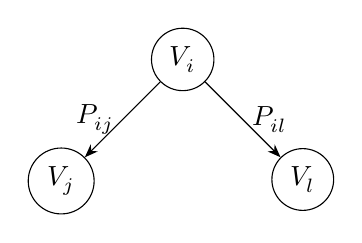
\begin{tikzpicture}
				\begin{scope}[every node/.style = {draw, circle},]
					\node [] (vi) at (0,0) {$V_{i}$};
					\node [below left  = 5em of vi] (vj) at (0,0) {$V_{j}$};
					\node [below right = 5em of vi] (vl) at (0,0) {$V_{l}$};
				\end{scope}

				\begin{scope}[>={Stealth}]
					\path [->] (vi) edge node[left, midway] {$P_{ij}$} (vj)
					           (vi) edge node[right, midway] {$P_{il}$} (vl);
				\end{scope}
			\end{tikzpicture}
			\caption{Граф алгоритму}
			\label{fig:graph-alg}
		\end{figure}

		Наприклад, нехай оператор~$i$ породжує перехід до~оператора~$j$ при~від'\-єм\-но\-му значенні деякої змінної~$Х$ та~до~оператора~$l$ при~додатному значенні~$Х$~(рис.~\ref{fig:graph-alg2}). Якщо відомо, що~величина~$Х$ рівномірно розподілена в~діапазоні~$(-1, 3)$, то~з~імовірністю~\num{0.25} її~знак є~від'\-єм\-ним та~з~імовірністю~\num{0.75}~— додатним. З~цього витікає, що~перехід до~оператора~$j$ відбувається з~ймовірністю~$P_{ij} = \num{0.25}$ та~перехід до~оператора~$l$~— з~імовірністю~$P_{il} = \num{0.75}$.

		\begin{figure}[!htbp]
			\centering
			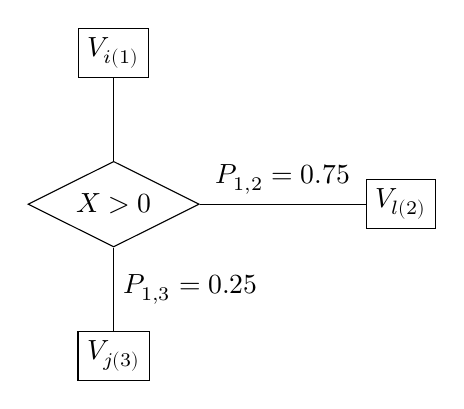
\begin{tikzpicture}
				\begin{scope}[every node/.style = {draw}]
					\node [] (vi1) at (0, 0) {$V_{i(1)}$};
					\node [diamond, aspect = 2, below = 3em of vi1] (xover0) {$X > 0$};
					\node [right = 6em of xover0] (vl2) {$V_{l(2)}$};
					\node [below = 3em of xover0] (vj3) {$V_{j(3)}$};
				\end{scope}

				\begin{scope}
					\path[-] (vi1)    edge node {} (xover0)
									 (xover0) edge node [above, midway] {$P_{1,2} = \num{0.75}$} 
									               node [below, near start] {Так} (vl2)
														edge node [right, midway] {$P_{1,3} = \num{0.25}$}
														     node [left , near start] {Ні} (vj3);
				\end{scope}
			\end{tikzpicture}
			\caption{Умовний оператор на графі алгоритму}
			\label{fig:graph-alg2}
		\end{figure}

		Для~операторів циклу ймовірність переходу визначається кількістю циклів. Наприклад, оператор циклу повинен виконуватися 9~разів, в~цьому випадку ймовірність виходу з~цикла~$P_{ij} = \num{0.1}$, а~ймовірність виконання циклу~$P_{ij} = \num{0,9}$. Якщо за~оператором~$і$ обов'\-яз\-ко\-во виконується оператор~$j$, то~$P_{ij} = 1$.

		Нехай $N_{1}, \dots, N_{k-1}$~— середнє число звернень до~операторів~$V_{1}, \dots, V_{k-1}$ за~один прогін алгоритму, $k_{i}$~— число операцій, які~складають оператор~$і$. У~такому випадку характеристики трудомісткості можуть бути обчислені таким чином: визначаємо середнє число процесорних операцій, що~виконуються при~одному прогоні алгоритму:
		\begin{IEEEeqnarray}{c}
			\label{eq:cpu-op-avg}
			\theta \leqslant \sum_{V_{oi}} n_{i} k_{i}.
		\end{IEEEeqnarray}
		Після цього визначаємо середнє число звернень до~файлу~$F_{h}$:
		\begin{IEEEeqnarray}{c}
			\label{eq:file-calls-avg}
			N_{h}  = \sum_{i = 1}^{V_{i}} n_{i}, \quad h = 1, \dots, H.
		\end{IEEEeqnarray}
		Потім визначаємо~середню кількість інформації, що~передається при~одному зверненні до~файла~$F_{h}$:
		\begin{IEEEeqnarray}{c}
			\label{eq:file-calls-byte-avg}
			\theta_{h}  = \frac{1}{N_{h}} \sum_{k = 1}^{V_{i}} n_{i} l_{i}, \quad h = 1, \dots, H,
		\end{IEEEeqnarray}
		де~$l_{i}$~— середня кількість інформації, яка передається при~виконанні оператора~$i$. 

		Значення~$N_{1}, \dots, N_{k - 1}$ визначаються роз\-в'я\-зком системи лінійних алгебраїчних рівнянь, канонічний запис яких має вигляд:
		\begin{IEEEeqnarray}{c}
			\label{eq:sys}
			\left\{ \,
			\begin{IEEEeqnarraybox}[][c]{rCrCrCrCl}
				\IEEEstrut
				(P_{11}-1)n_{1}  &+& P_{21} n_{2}       &+& \dots &+& P_{(k-1)1} n_{k-1} &=& -1,\\*
				P_{12} n_{1}     &+& (P_{22} – 1) n_{2} &+& \dots &+& P_{(k-1)2} n_{k-1} &=& 0, \\*
												 & &                    & & \dots \\*
				P_{1(k-1)} n_{1} &+& P_{2(k-1)} n_{2}   &+& \dots &+& (P_{(k-1)(k-1)} – 1) n_{k-1} &=& 0.
				\IEEEstrut
			\end{IEEEeqnarraybox}
			\right.
		\end{IEEEeqnarray}

		У виразі~\eqref{eq:cpu-op-avg} підсумовування виконується для~всіх вершин, які~належать до~основних операторів. У~виразах~\eqref{eq:file-calls-avg} і~\eqref{eq:file-calls-byte-avg}~— для~всіх вершин, що~відображають звернення до~даного файлу. 

		При~формуванні коефіцієнтів системи~\eqref{eq:sys} необхідно звернути увагу на~те, що~коефіцієнти~$P_{ij}$ записуються не~по~рядках, а~по~стовпцях, тобто, наприклад, на~місці другого елемента першого рядка стоїть елемент з~індексом 21, а~не~коефіцієнт з~індексом~12 матриці переходів.

		Визначивши за~формулами~\eqref{eq:cpu-op-avg}, \eqref{eq:file-calls-avg} і~\eqref{eq:file-calls-byte-avg} величини~$\theta$, $N_{h}$, $\theta_{h}$, можна визначити середню трудомісткість етапу рахування, на~основі якої виконується оцінка оптимальної швидкодії процесора.

		Середня трудомісткість етапу рахування визначається за~формулою:
		\begin{IEEEeqnarray}{c}
			\theta_{\text{О}} = \frac{\theta}{N},
		\end{IEEEeqnarray}
		де~$N$~— сума середнього числа~$N_{i}$ звернень до~основних операторів~$S_{\text{О}}$, тобто:
		\begin{IEEEeqnarray}{c}
			N = \sum_{i = 1}^{V_{\text{О}i}} n_i,
		\end{IEEEeqnarray}

	\section{Вихідні дані}
		Вихідними даними для лабораторної роботи є схема алгоритму~(рис.~\ref{fig:flowchart}). 

		\begin{figure}[!htbp]
			\centering
			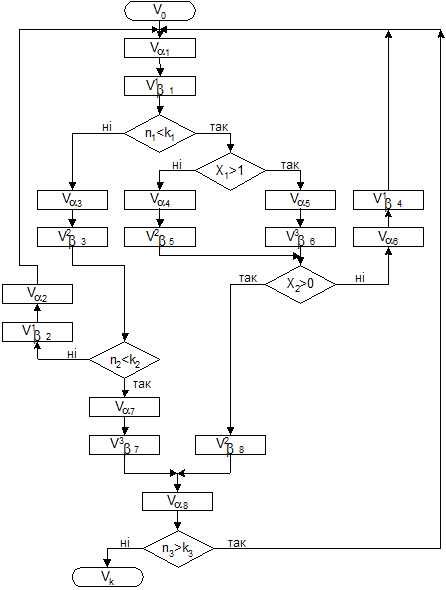
\includegraphics[height = 25\baselineskip]{./assets/y03s02-compsys-lab-01-p01.png}
			\caption{Схема алгоритму}
			\label{fig:flowchart}
		\end{figure}

	\section{Запитання для~самоперевірки}

		\subsection{Дати визначення поняттю «трудомісткість алгоритмів»}
			Трудомісткість алгоритмів~— це кількість обчислювальної роботи, яка~необхідна для~реалізації цих алгоритмів на~обчислювальній системі. Трудомісткість оцінюється кількістю операцій, що~виконуються з~метою обробки вводу та~виводу інформації в~процесі роз\-в'я\-за\-ння задачі.

		\subsection{Для чого використовують поняття «трудомісткість алгоритмів»}
			Поняття «трудомісткість алгоритмів» використовують для оцінки потреб у~часі, пов'\-я\-за\-них з~періодом роботи сукупності пристроїв обчислювальних систем.

		\subsection{У вигляді чого можна подати обчислювальний процес?}
			Обчислювальний процес подають у~вигляді моделі, яка~несе в~собі інформацію тільки про~властивості самого процесу. При~оцінці трудомісткості обчислювальний процес можна подати у~вигляді послідовності операторів. 

		\subsection{Сформулювати вимоги до~моделі обчислювального процесу}
			Модель обчислювального процесу повинна:
			\begin{enumerate}[itemsep = 1\baselineskip]
				\item Визначати порядок проходження алгоритмів запитів на~кожен з~видів обслуговування~— рахування та~ввод-вивід інформації.
				\item Визначати трудомісткість обслуговування запитів~— кількість операцій, яку~повинен виконати процесор при~обслуговуванні запиту на~рахування, та~кількість символів інформації, що~вводиться або~виводиться. 
				\item Відповідати реальним процесам з~точністю до~збігу, як~найменше, математичних очікувань їх~однойменних характеристик. 
			\end{enumerate}

		\subsection{Які розрізняють типи операторів алгоритму?}
			Розрізняють 3 типи операторів алгоритму: 
			\begin{enumerate}[itemsep = 1\baselineskip]
				\item Функціональні~— задають сукупність обчислювальних операцій. 
				\item Оператори переходу~— задають правила вибору одного з~можливих шляхів розвитку обчислювального процесу. 
				\item Оператори звернення до файлів~— відображають процес обміну інформацією із~зовнішніми пристроями. 
			\end{enumerate}

		\subsection{Якими параметрами можна охарактеризувати трудомісткість алгоритму?}
			Трудомісткість алгоритму можна охарактеризувати такою сукупністю параметрів: $Q$~— середня кількість процесорних операцій, які виконуються за одну реалізацію алгоритму, $N_1, \dots, N_{h}$~— середній час звернення до файлів $F_{1}, \dots, F_{h}$, $\theta_1, \dots, \theta_{h}$~— середня кількість байтів, що передається за одне звернення до файлів $F_{1}, \dots, F_{h}$ відповідно. 


	\section{Висновок}
		Виконуючи дану лабораторну роботу, ми ознайомились з~моделями обчислювальних процесів. 

\end{document}

